\begin{frame}{Result}
  
  { \centering
    $d(K^-, p)"\pi^-\Sigma^0"$ \&  $d(K^-, p)"\pi^-\Lambda"$ $I=1$ channel
  }
  \begin{tabular}{ccc}
    \begin{minipage}{0.2\hsize}
      \begin{figure}
        \scriptsize
        $d(K^-, p)"\pi^-\Sigma^0"$
        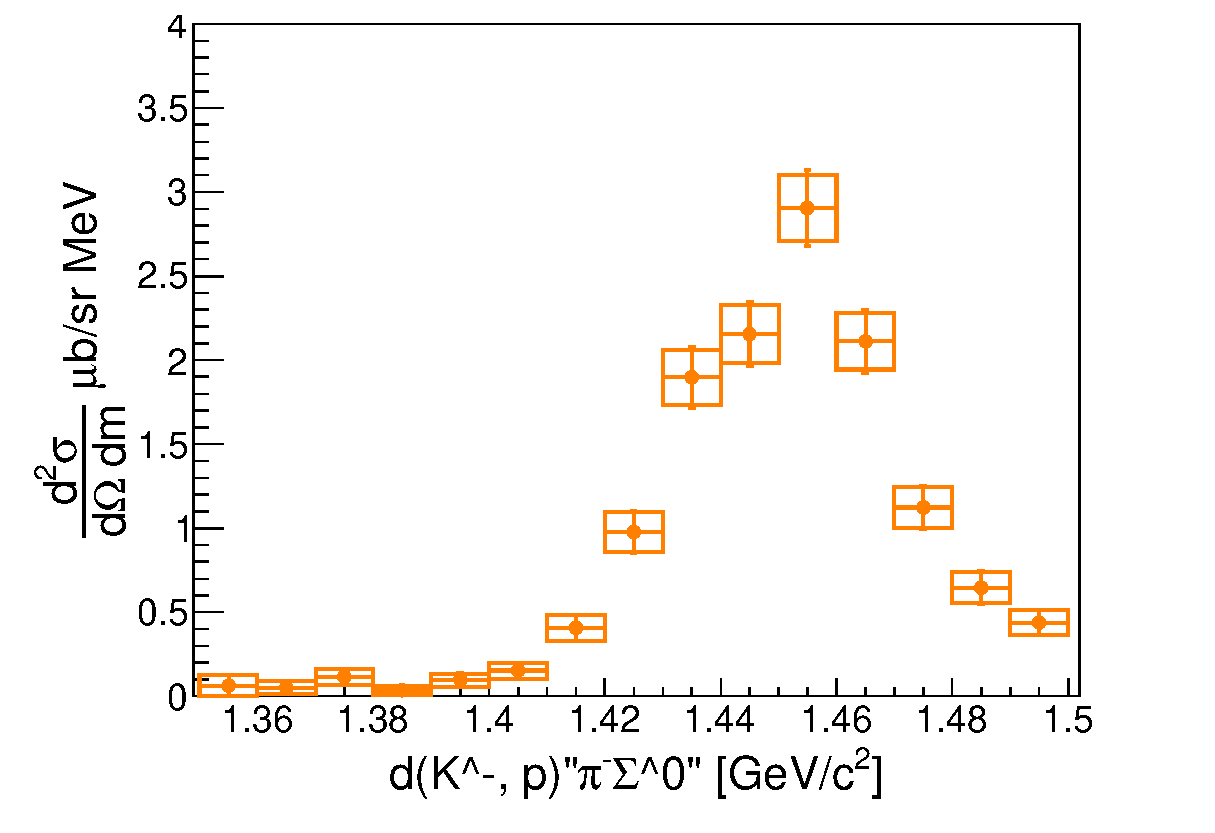
\includegraphics[width=2.5cm]{../pic/Run68/KP_ana/pimS0_CS_zoom.eps}
      \end{figure}
    \end{minipage}
    \begin{minipage}{0.2\hsize}
      \begin{figure}
        \scriptsize
        $d(K^-, p)"\pi^-\Lambda"$
        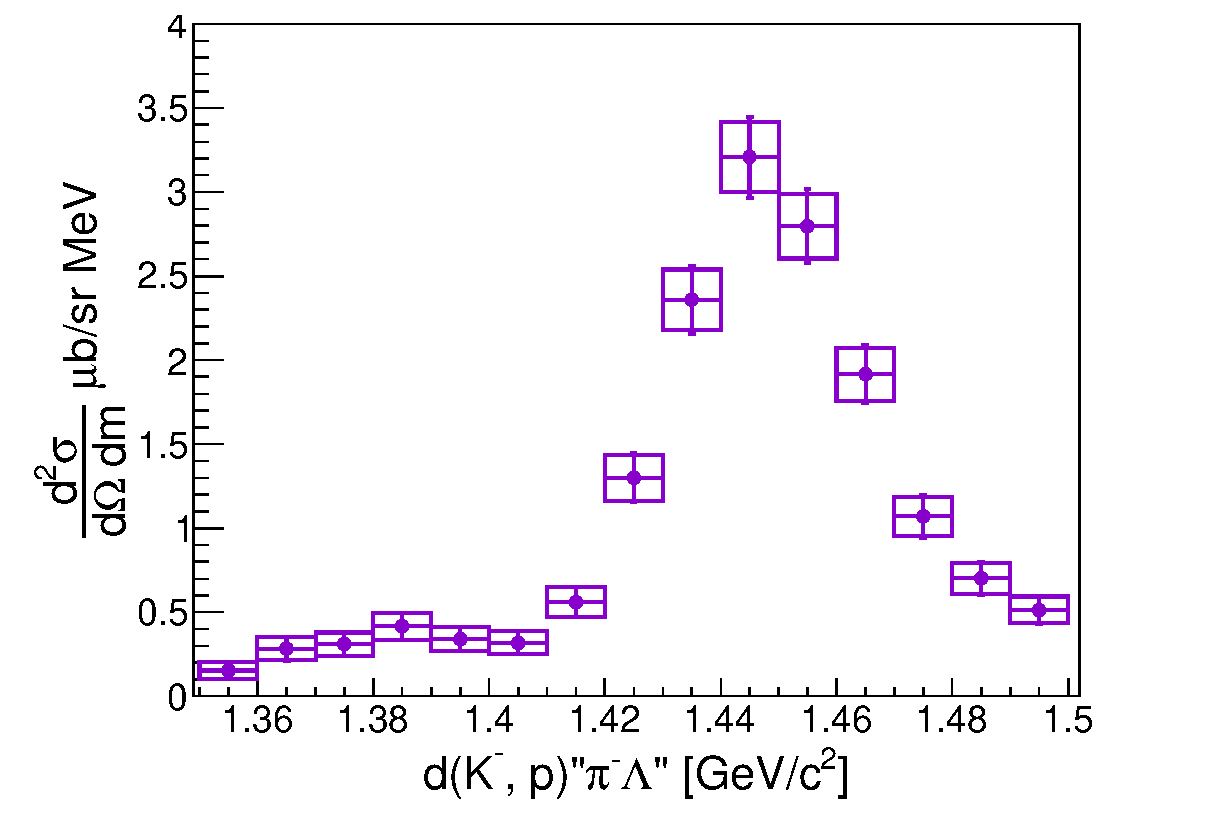
\includegraphics[width=2.5cm]{../pic/Run68/KP_ana/pimL_CS_zoom.eps}
      \end{figure}
    \end{minipage}
    \begin{minipage}{0.6\hsize}
      \scriptsize
      $I=1$, $d(K^-, p)"\pi^-\Sigma^0/\Lambda"$ scattering amplitude were \\suppressed in the $\bar{K}N$ threshold.
    \end{minipage}
  \end{tabular}

  { \centering
    $d(K^-, n)"n K^0"$ Quasi-elastic 
  }  
  \begin{tabular}{ccc}
    \begin{minipage}{0.2\hsize}
      \begin{figure}
        \scriptsize
        $d(K^-, n)"n K^0"$
        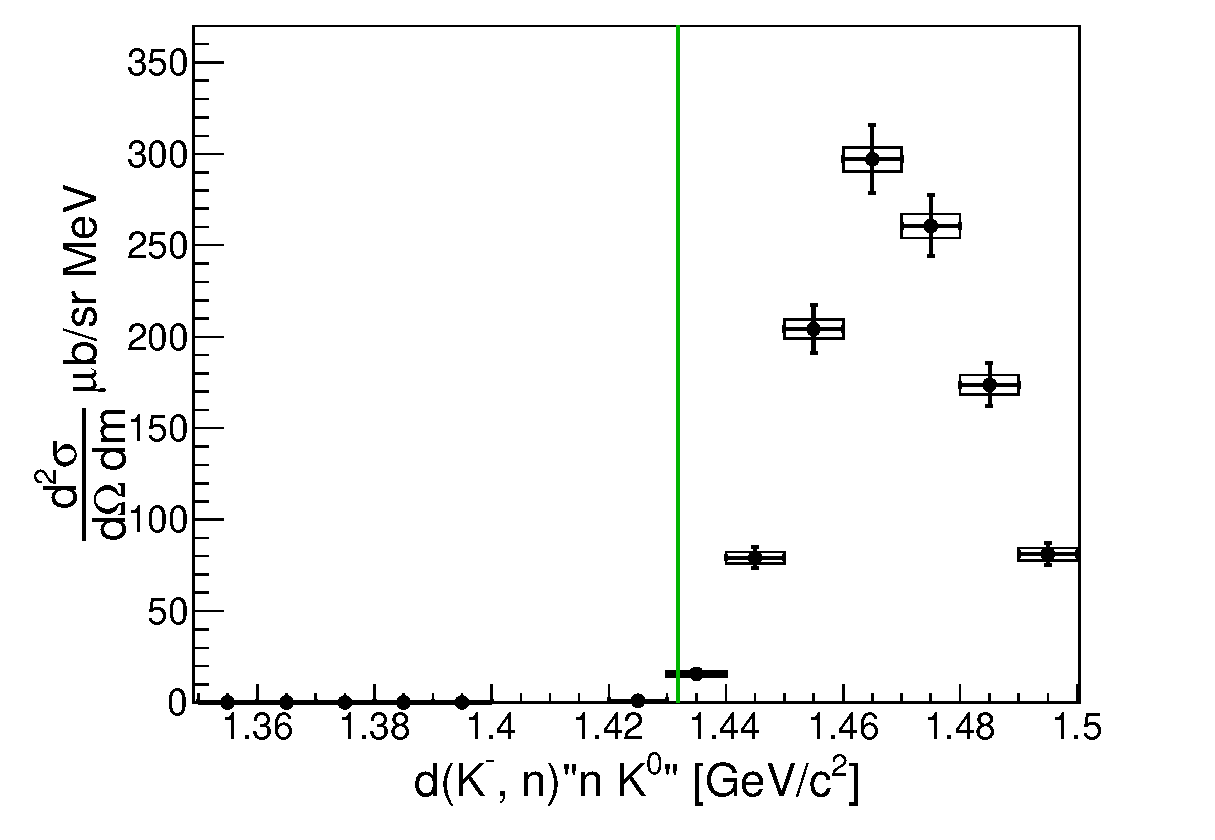
\includegraphics[width=2.5cm]{../pic/Run78/QE/K0_CS.eps}
      \end{figure}
    \end{minipage}
    \begin{minipage}{0.2\hsize}
      \begin{figure}
        \scriptsize
        $n_{detect} K^0$ IM
        \includegraphics[width=2.5cm]{../pic/Run78/KN_ana/fit_KN_IM_npipi_K0_ts_L1520.eps}
      \end{figure}
    \end{minipage}
    \begin{minipage}{0.6\hsize}
      \scriptsize
      $d(K^-, n)"n K^0"$ spectrum look quasi-elastic 1-step \\ $K^-d \rightarrow n K^0 n_{spec}$ reaction.\\
      In about 12\% of them, recoiled $\bar{K}$ scatters with \\ residual neucleon was occupied.\\
      In about 8\% of them, n $\Lambda(1520)$ production was occupied.\\
    \end{minipage}
  \end{tabular}

  { \centering
    $d(K^-, n)"\pi^{\mp}\Sigma^{\pm}"$ $I=0,1$ channel
  }  
  \begin{tabular}{ccc}
    \begin{minipage}{0.2\hsize}
      \begin{figure}
        \scriptsize
        $d(K^-, n)"\pi^{\mp}\Sigma^{\pm}"$
        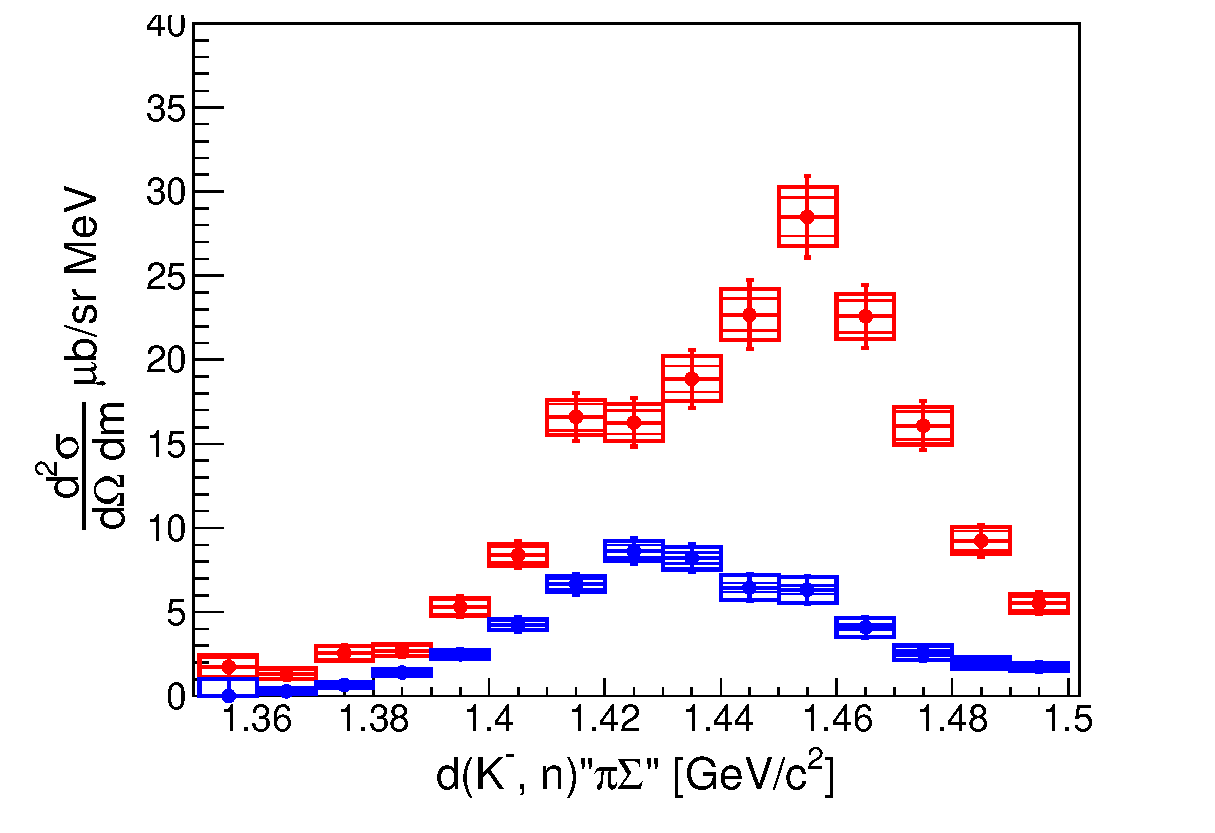
\includegraphics[width=2.5cm]{../pic/Run78/K0_ts_L1520/ChargeCS_after.eps}
      \end{figure}
    \end{minipage}
    \begin{minipage}{0.2\hsize}
      \begin{figure}
        \scriptsize
        $d(K^-, n)"\pi^{\mp}\Sigma^{\pm}"$ average
        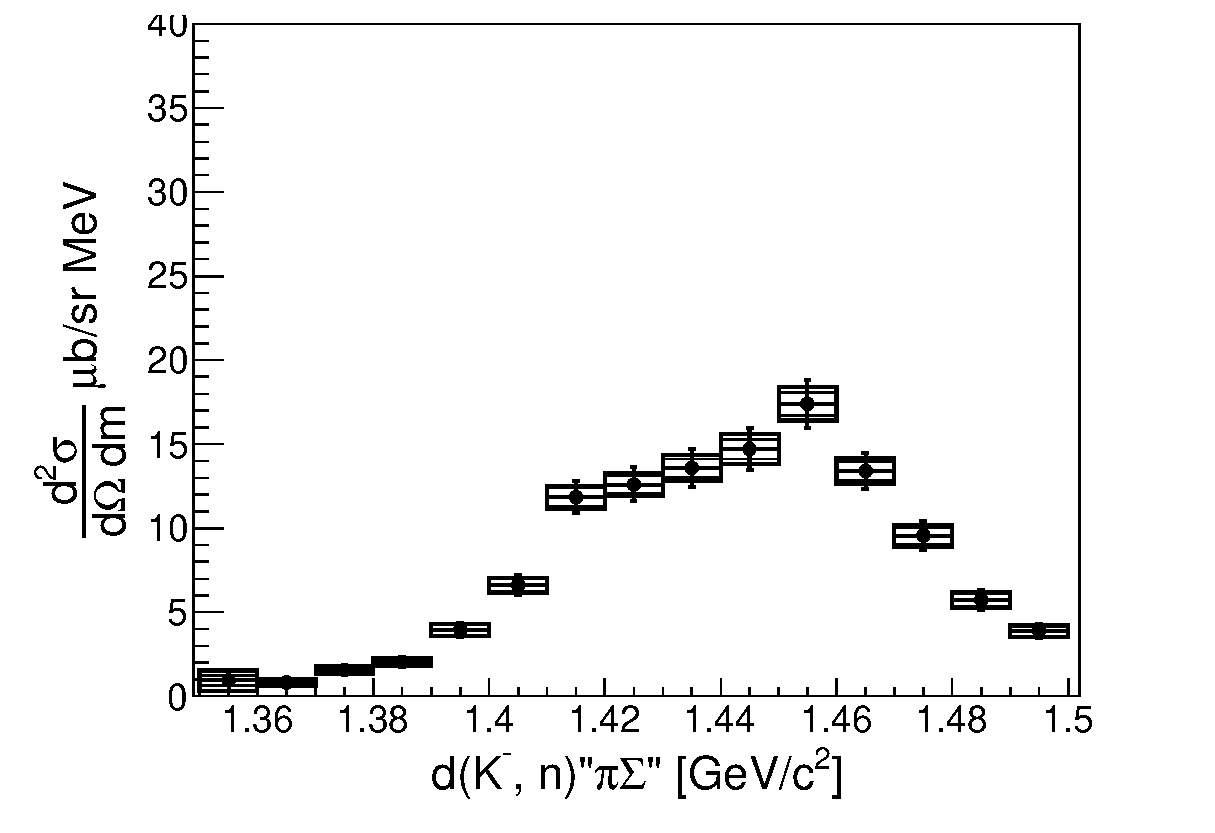
\includegraphics[width=2.5cm]{../pic/Run78/K0_ts_L1520/ChargeCS_ave_after.eps}
      \end{figure}
    \end{minipage}
    \begin{minipage}{0.6\hsize}
      \scriptsize
      Interferance term of $d(K^-, n)"\pi^{\mp}\Sigma^{\pm}"$ was observed.\\
      Scattering amplitude of about 5\% quasi-elastic was \\ obserbed above the $\bar{K}N$ threshold. \\
      Large scattering amplitude was observed even in \\ the $\bar{K}N$ threshold.
    \end{minipage}
  \end{tabular}
\end{frame}
